% =========================================================
% CHAPTER 11: UML MODELING
% =========================================================
\chapter{UML Modeling}
\label{chap:uml_modeling}

\section{Introduction to System Modeling}
Unified Modeling Language (UML) diagrams provide standardized visual representations of system actors, object interactions, behavioral states, and static architectural structures.

\section{Use Case Diagram}
Figure~\ref{fig:uml_use_case} illustrates the UML Use Case Diagram defining the operational boundaries between regular retail customers and SOC security administrators.

\begin{figure}[htbp]
    \centering
    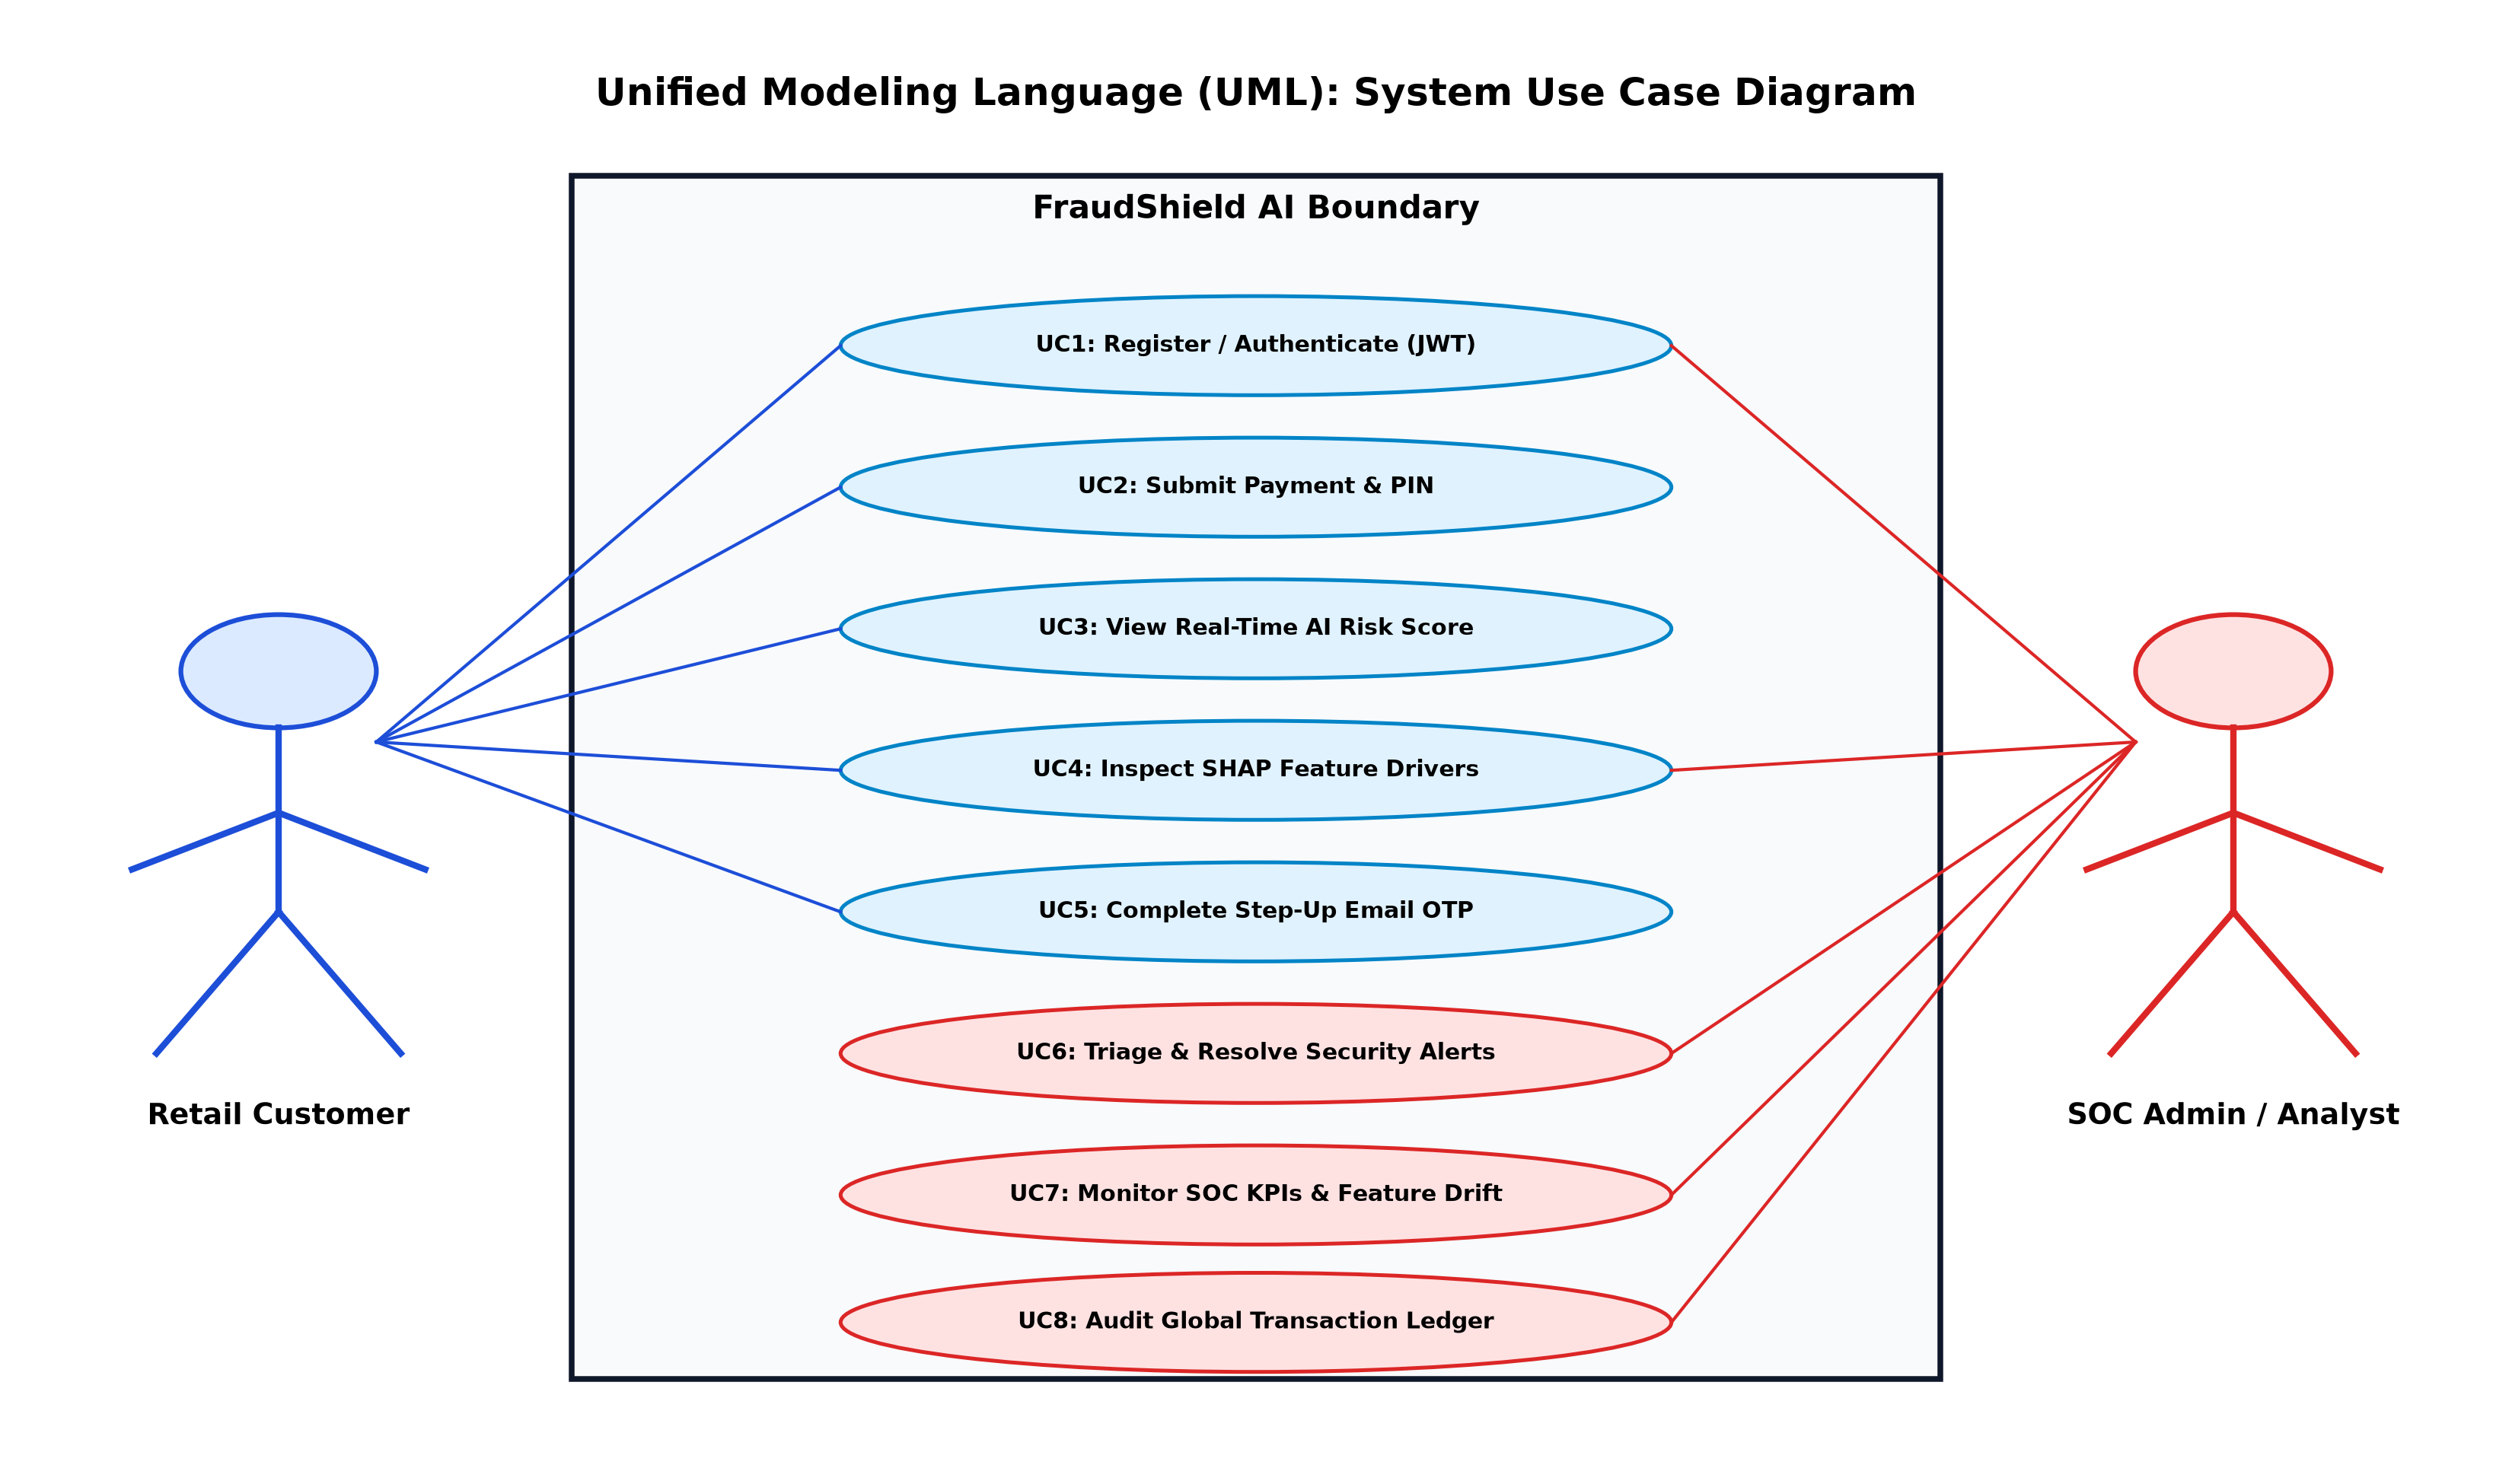
\includegraphics[width=0.95\textwidth]{figures/uml_use_case.png}
    \caption{UML Use Case Diagram: Customer and Administrator Interactions}
    \label{fig:uml_use_case}
\end{figure}

\subsection{Use Case Descriptions}
\begin{itemize}
    \item \textbf{UC1 (Authenticate)}: Customer or Admin logs into the system with credentials, receiving a signed JWT access token.
    \item \textbf{UC2 (Submit Payment \& PIN)}: Customer initiates payment, specifying beneficiary, amount, and numeric Payment PIN.
    \item \textbf{UC3 \& UC4 (View AI Risk \& SHAP Explanation)}: Client receives the real-time risk score ($0-100$) and inspects natural language and visual feature attribution bars.
    \item \textbf{UC5 (Complete Step-Up Email OTP)}: For held transactions (\textit{MEDIUM} / \textit{HIGH}), customer inputs the 6-digit verification code delivered to their registered email address.
    \item \textbf{UC6, UC7 \& UC8 (SOC Operations)}: Security officers investigate queued alerts, resolve incidents with audit notes, monitor feature drift, and review global transaction ledgers.
\end{itemize}

\section{Sequence Diagram — Transaction Lifecycle}
Figure~\ref{fig:uml_sequence} details the complete synchronous and asynchronous interaction flow across client JavaScript controllers, Flask REST APIs, ML inference pipelines, SHAP explainers, risk engines, and database stores.

\begin{figure}[htbp]
    \centering
    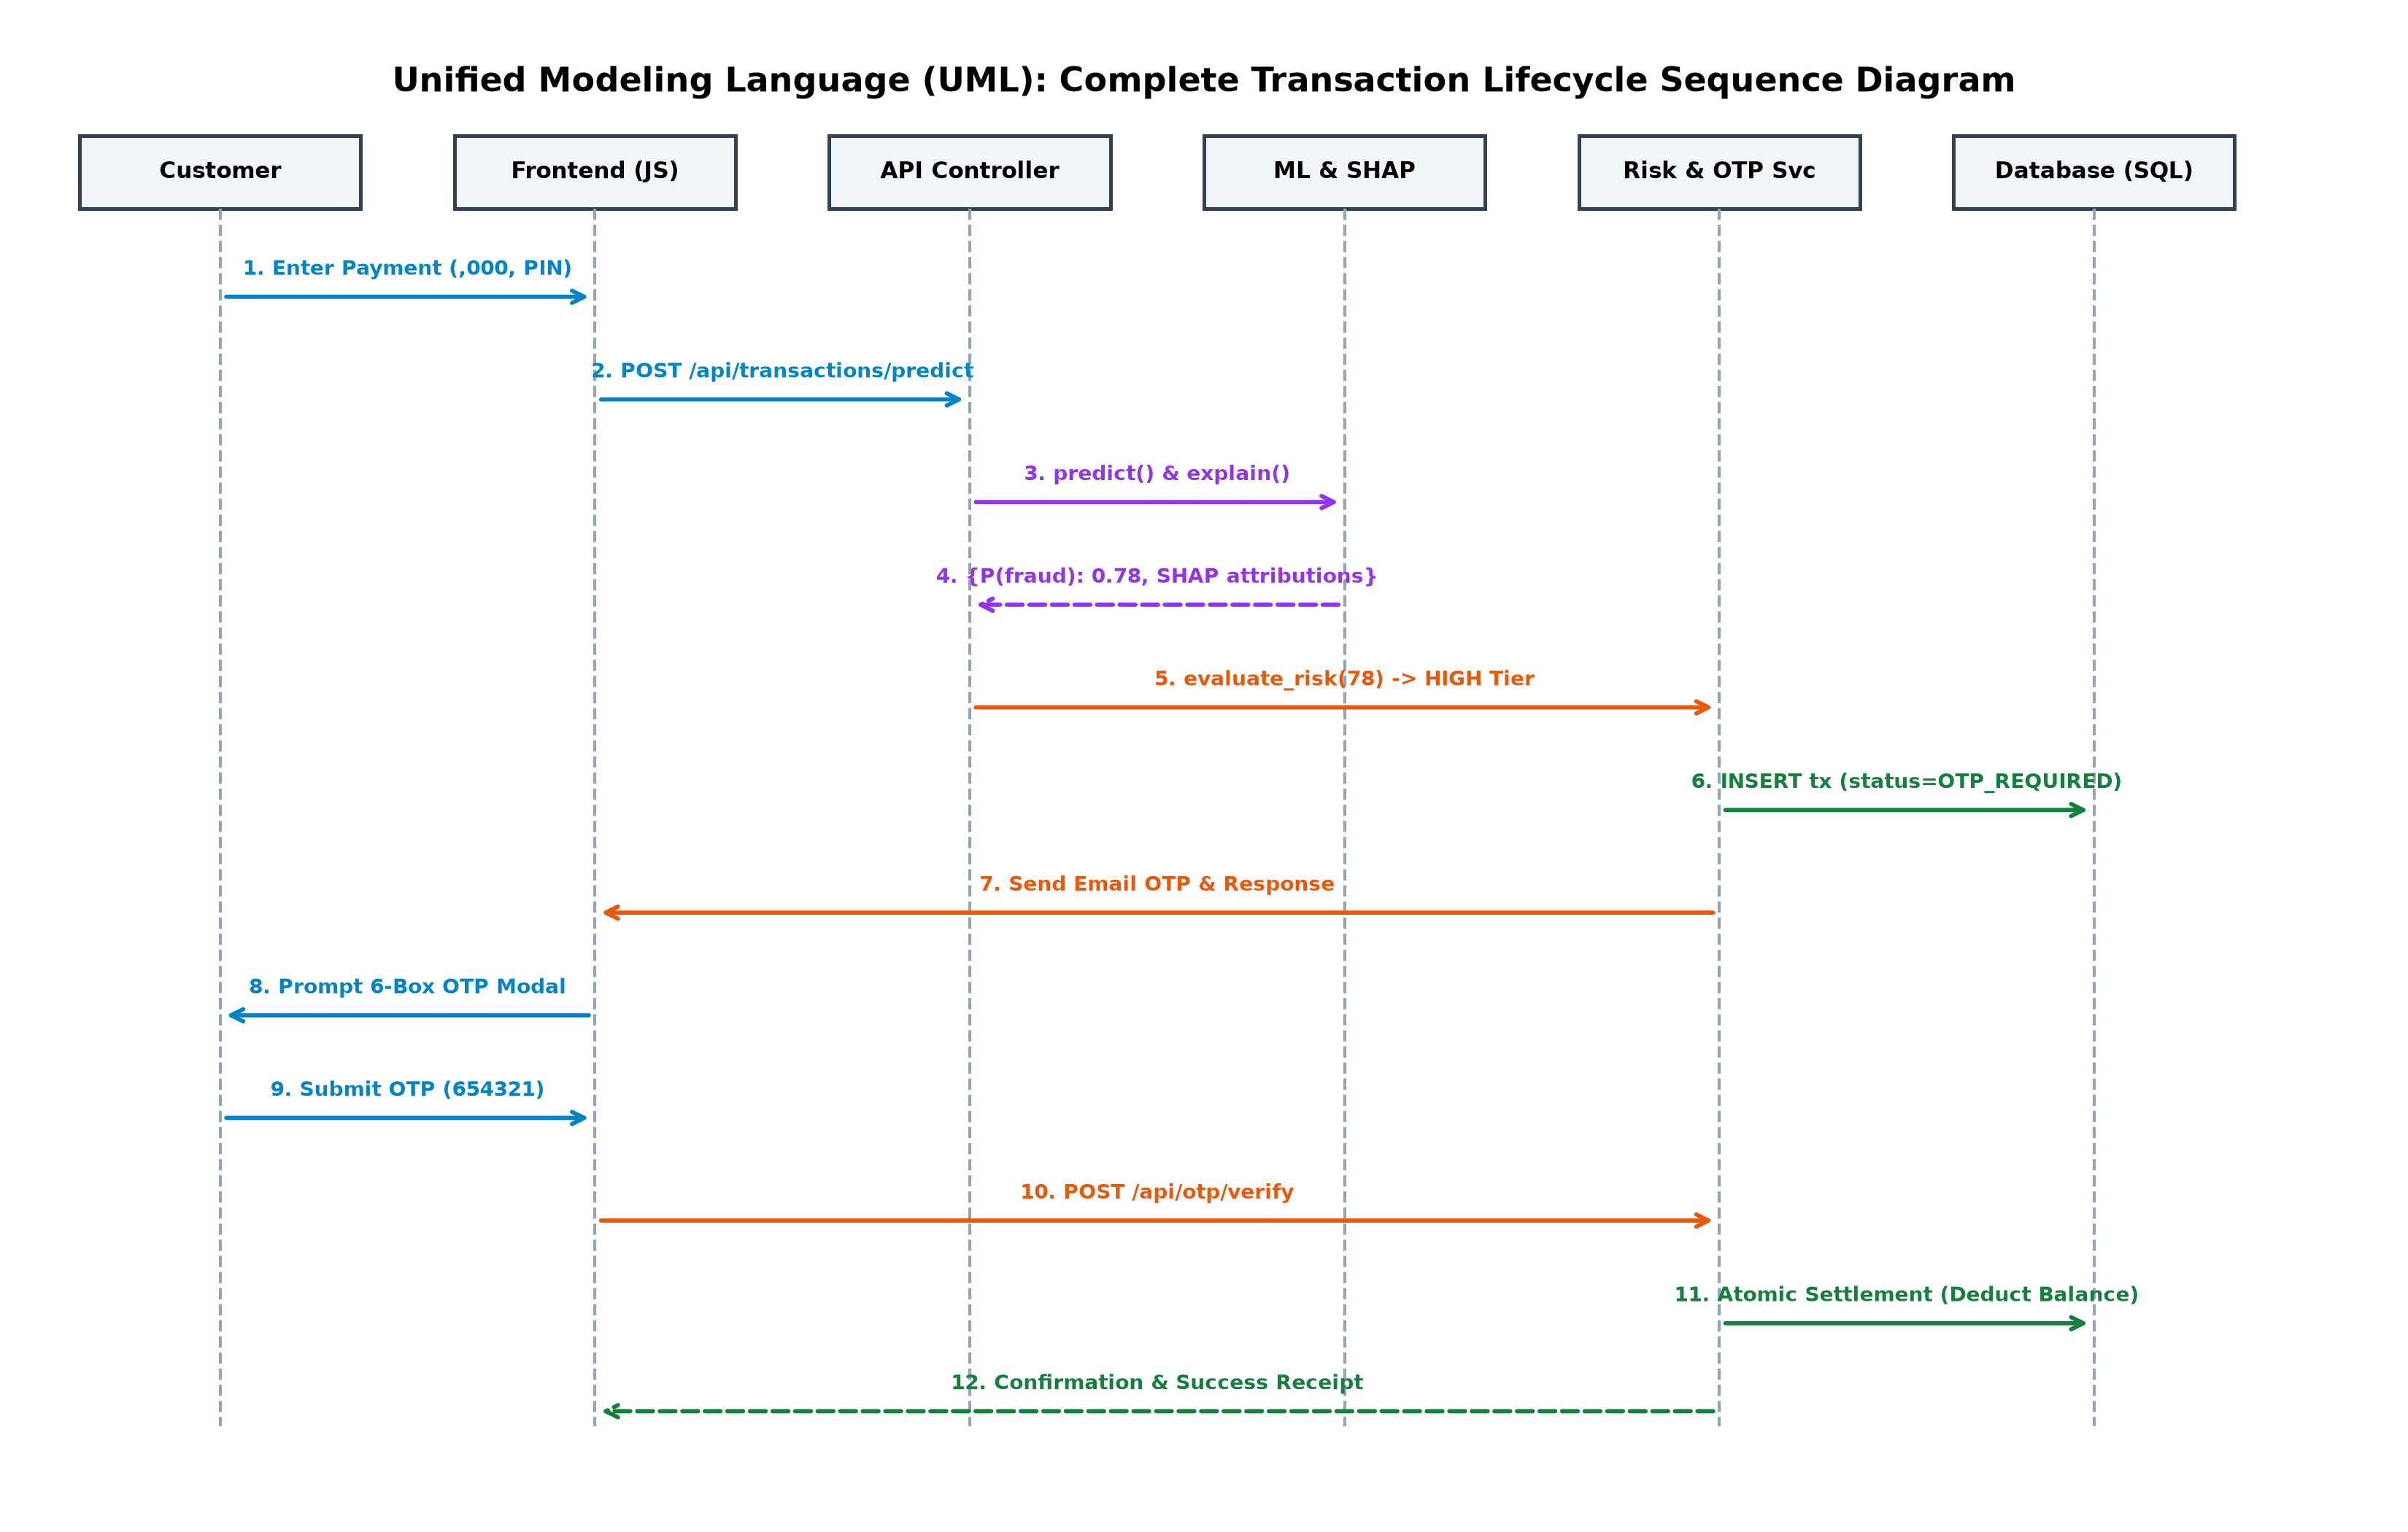
\includegraphics[width=0.95\textwidth]{figures/uml_sequence.png}
    \caption{UML Sequence Diagram: End-to-End Payment Evaluation \& Verification Flow}
    \label{fig:uml_sequence}
\end{figure}

\section{Class Diagram — Domain Object Architecture}
The core domain model encapsulates domain entities, service controllers, and helper abstractions:
\begin{itemize}
    \item \textbf{\texttt{User}}: Implements identity, cryptographic authentication (\texttt{check\_password()}, \texttt{verify\_pin()}), and account balance balance attributes.
    \item \textbf{\texttt{Transaction}}: Encapsulates transaction state, risk classification properties, and serialization methods.
    \item \textbf{\texttt{OTPChallenge}}: Manages one-time token lifecycles, expiration checks (\texttt{is\_expired()}), and attempt counter decrements.
    \item \textbf{\texttt{Alert}}: Encapsulates high-risk incident triage states and analyst audit notes.
    \item \textbf{\texttt{InferenceService} \& \texttt{ShapService}}: Singleton service classes that encapsulate the Random Forest classifier and SHAP TreeExplainer.
\end{itemize}

\section{Activity Diagram — 4-Tier Adaptive Security Routing}
The activity flow begins when the customer submits a payment request. The system validates syntax and balance, extracts 11 engineered features, executes Random Forest inference, calculates SHAP attributions, and computes the composite risk score. Depending on the score band:
\begin{itemize}
    \item If $\text{Score} \le 29$ (\textit{LOW}): Transaction settles instantly.
    \item If $30 \le \text{Score} \le 79$ (\textit{MEDIUM} / \textit{HIGH}): Transaction is held; Email OTP is generated; balance deduction is blocked until verification.
    \item If $\text{Score} \ge 80$ (\textit{CRITICAL}): Transaction is locked under review and routed to the SOC queue.
\end{itemize}

\section{Component and Deployment Architecture}
The physical deployment model utilizes a modular containerized topology where the client browser interacts with the Flask WSGI application server via HTTPS. The Flask application communicates with the local/cloud relational database (SQLite/MySQL) and triggers external SMTP relay connections over TLS (Port 587) for OTP email delivery.
